\documentclass[../main.tex]{subfiles}
\begin{document}
\section{Web challenges}

\subsection{Vote calculator}
With the Vote calculator challenge, the aim is to add up the votes and get the total.

Many counters in America need to see that the votes are counted correctly. Now it is up to you to calculate the votes.

You will have the opportunity to add up the votes that are given to you. But there is a way to manipulate the votes. Can you cope with this challenge?

\subsubsection{Vote calculator explained}

For this challenge, you'll get a PHP page. This will consist of a forum for the purpose of calculating votes. The intention is to find an exploit, which will show you the flag. The underlying code consists of a function called flag(). 

This function calculates the votes, but also contains the flag to be found. The intention for the hacker is to find the flag. A tip is given at the beginning, but the purpose is to manipulate with the eval(). 

The eval() code evaluates a string as PHP code. This construction is very dangerous because it allows execution of arbitrary PHP code. You could easily retrieve data that can be used for illegal purposes.

\subsubsection{Vote calculator write up}

At the beginning there will be a small tip.

The tip is:
80 + 108 + 97 + 121 + 32 + 119 + 105 + 116 + 104 + 32 + 69 + 118 + 97 + 108 

This tip is an ASCII value that you can convert to a string. But the intention is to mislead the hacker a little. He would first think that you can add this up with the vote calculator. Which is correct but after some time he should know that this is actually a message. Once you convert the ASCII value to a string. It would say "play with eval code". 

The intention is to print the flag. This can be done by executing codes by Eval(). Eval() is very dangerous in PHP because it can execute code without asking the user's permission. For example, you can request folders and personal information. In this case, the purpose is to print the variable. Because the flag is defined as a variable you would see the flag immediately. 

You can do this by executing this command as you see on the picture.

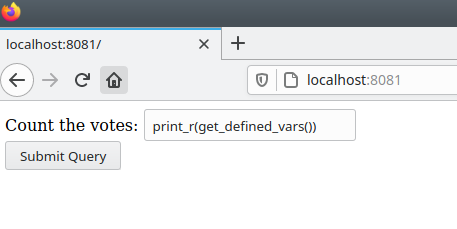
\includegraphics[width=\linewidth]{images/Boyan/challenge1_boyan.PNG}
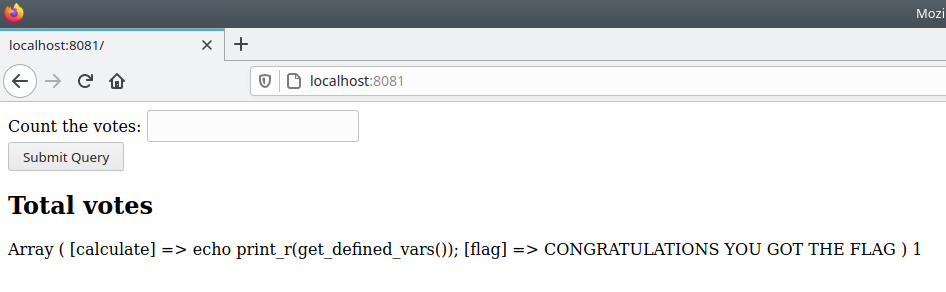
\includegraphics[width=\linewidth]{images/Boyan/challenge1_2_boyan.PNG}

After executing this command you will see the flag immediately. 

\subsection{Log in manager}

One of the President's candidates is eager to win and is doing everything to be in charge. To do so, he hires a hacker. 

The candidate would like to see the progress of the votes. 

But only the manager can see this. Can you be the secret hacker who can break into the system?

\subsubsection{Log in manager explained}

The purpose of this challenge is to find a txt file. Which you are trying to hack. You will get an HTML page with a login button. This will then assign you to the login page. There you will have to find out, how to find the txt file. 

Once you have found the txt file you will see that you will get an encrypted code combination which you will have to execute with the John the Ripper command. Once you have done this you will get the secret password. 

\subsubsection{Log in manager write up}

If you do your own research, you would conclude that you can't find anything on the website. The right step to take is to execute the dirb command on the website. Dirb will look at the existing folders and hidden files. 

Commands:
\begin{lstlisting}
dirb http://localhost:8080 -o dirlogin.txt
\end{lstlisting}
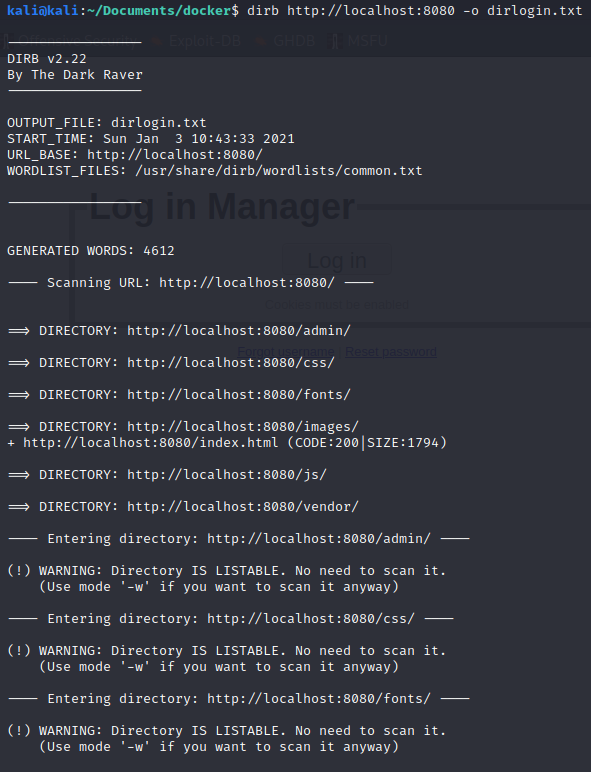
\includegraphics[width=\linewidth]{images/Boyan/challenge2_1_boyan.PNG}

When you execute the command. You will see that it has found several folders. The most interesting one is the admin folder. You might find something here. The output should also be sent in an output file. 

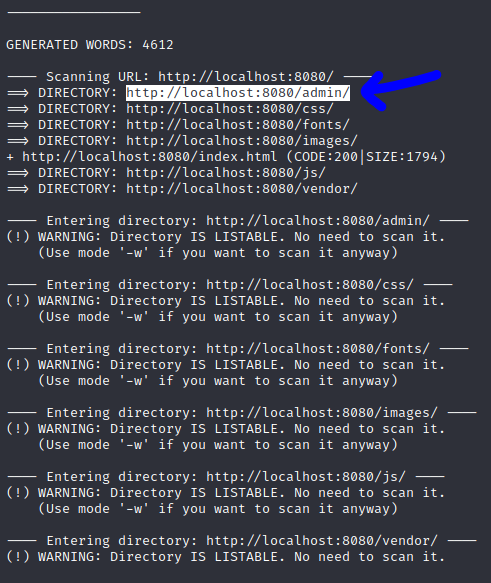
\includegraphics[width=\linewidth]{images/Boyan/challenge2_2_boyan.PNG}
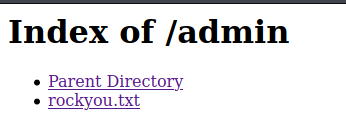
\includegraphics[width=\linewidth]{images/Boyan/challenge2_5_boyan.PNG}
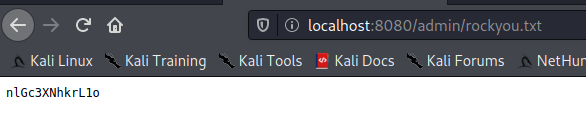
\includegraphics[width=\linewidth]{images/Boyan/challenge2_3_boyan.PNG}
Then click on the link "http://localhost:8080/admin". You can immediately see what this folder has to hide. As you can see there is a "rockyou.txt" file. Once we open this you can see the encrypted code which you need to run afterwards with John the Ripper command. 

Once you have done this, you should have cracked the secret code. The image shows the correct code that I have executed before. 

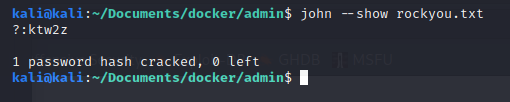
\includegraphics[width=\linewidth]{images/Boyan/challenge2_4_boyan.PNG}


\subsection{Message board}

Because of the fact that traditional communication techniques are monitored very hard by counterparties. The team of the presidential candidate developed an app to communicate securely. 

Our system is called a message board. In this way, the candidates in the field can forward information to our head office. You could then view all messages on a "secret" page.

To access this message board, you need a special certificate. But the developers have made a mistake when they created the app. Can you find the exploit in our system before the opposition found out about it?

\subsubsection{Message board explained}

The purpose of this challenge is to find a common exploit used by Flusk, called Server Side Template Injection.

\textit{Template engines are designed to generate web pages by combining fixed templates with volatile data. Server-side template injection attacks can occur when user input is concatenated directly into a template, rather than passing in as data. This allows attackers to inject arbitrary template directives in order to manipulate the template engine, often enabling them to take complete control of the server.}

Because data is often transferred from one web page to another, it may go wrong when rendering the content.

\subsubsection{Message board write up}

This challenge contains a very important hint in the URL name, namely "ssti". That would be enough to understand that we are going to run Server Side Template Injection.

Furthermore, the app has been specially designed in such a minimalist way that only 1 payload will be available. 

The payload \begin{verbatim}
{{config.__class__.__init__.__globals__['os'].popen('cat /root/flag.txt').read()}}
\end{verbatim}

All other payloads could perform basic functions but rendering the content will not work.



\end{document}